\documentclass[a4paper,12pt]{article}
\usepackage{graphicx}
\usepackage{rotating}
\usepackage{bbding}
\begin{document}

\title{System Validation Project Report}
\author{
	Suryansh Sharma \\ 
	\texttt{S.sharma-13@student.tudelft.nl}
 	\and 
	Snehal Jauhri \\
	\texttt{S.jauhri@student.tudelft.nl} 
	\and
	Suhail Nogd \\
	\texttt{S.T.S.nogd@student.tudelft.nl} 	
	 \and 
	Apoorva Arora\\
	\texttt{A.Arora-1@student.tudelft.nl} 
}

\date {\today}
\maketitle
\newpage
\tableofcontents
 
\newpage
\section{Introduction}
This is a project done as part of TU Delft's IN4387 System Validation course. The project concerns designing, modelling and validating a controller for a Transfer system in an Industrial Silicon Wafer production plant.
\\
\\The system consists of a UV Lamp that projects a design onto a wafer inside a vacuum chamber. The wafers are transferred to the Lamp via two Airlocks. The wafers are handled by robots from their initial position on the Input stacks to their final position on the Output stacks. The wafers move along the production line from their Initial state (on the Input Stacks), are printed on by the Lamp and reach the Final state (on the Output stacks).
\\
\\Described here is the documentation for the modelling of the above system in mcrl2 and it's verification using Modal $\mu$ calculus. Section 2 describes the System and Functional Requirements. Section 3 is dedicated to the interactions between the various subsystems defined in section 2. The architecture of the resulting system is shown in section 4. In section 5 the requirements are translated into Modal S$\mu$-calculus. Section 6 describes the modelling process. In section 7 the model is verified with the translated requirements. The final conclusions are presented in section 8.

\section{Requirements}

\subsection{System Components}
The system consists of the following physical components:
\begin{itemize}
\item Lamp/Projector: L
\item Inner Doors: DI1, DI2
\item Outer Doors: DO1, DO2
\item Input Stacks: I1, I2
\item Output Stacks: O1, O2
\item Airlocks: AL1, AL2
\item Outer Robots: R1, R2
\item Inner Robot: R3
\end{itemize}


\subsection{System Requirements}
The behaviour of the system can be understood by listing the following requirements:

\begin{enumerate}
%1
\item Once a wafer is picked up from an Input Stack, it eventually gets printed and placed on the Output Stack if the Output Stack is not full. (\textbf{As long as the wafer can move through the production process, it will.}) \textbf{[Liveness]}
%2
\item Once a wafer is picked up from an Input Stack (I1 or I2), the next wafer from that Input Stack gets picked up only after the previous wafer has been printed and placed on the corresponding Output Stack. \textbf{[Safety]}
%3
\item The Outer Robots (R1 and R2) should not place a wafer on the Input Stacks (I1 and I2). \textbf{[Safety]}
%4
\item The Outer Robots (R1 and R2) should not pickup a wafer from an empty Input Stack. \textbf{[Safety]}
%5
\item Once an \textbf{unprocessed} wafer is picked up from its Input Stack (I1 or I2) by the Outer Robots (R1 and R2), it gets placed only in it's corresponding Airlock (A1 or A2). \textbf{[Safety]}
%6
\item The Outer Robots (R1 and R2) must not pickup an \textbf{unprocessed} wafer from the Airlocks (AL1 and AL2). \textbf{[Safety]}
%7
\item The Outer and Inner Doors of the Airlocks must not be opened at the same time \textbf{[Safety]}
\begin{enumerate}
    \item The Inner Door (DI1) must not be opened if the Outer Door(DO1) is open for Airlock (AL1).

    \item The Inner Door (DI2) must not be opened if the Outer Door(DO2) is open for Airlock (AL2).

    \item The Outer Door (DO1) must not be opened if the Inner Door(DI1) is open for Airlock (AL1).

    \item The Outer Door (DO2) must not be opened if the Inner Door(DI2) is open for Airlock (AL2).

\end{enumerate}
%8
\item Once an \textbf{unprocessed} wafer is picked up from an Airlock by the Inner Robot (R3), the wafer gets placed on the Lamp. \textbf{[Liveness]}
%9
\item The Inner Robot (R3) will only pickup a \textbf{finished} i.e. printed wafer from the Lamp (L). \textbf{[Safety]}
%10
\item The Inner Robot (R3) will not place the \textbf{finished} wafer again on the Lamp (L). \textbf{[Safety]}
%11
\item Once a \textbf{finished} wafer is picked up from the Lamp by the Inner Robot (R3), the wafer gets placed in its corresponding Airlock. \textbf{[Liveness]}
%12
\item The Inner Robot (R3) should not pickup a \textbf{processed} wafer from the Airlocks. \textbf{[Safety]}
%13
\item Once a \textbf{finished} wafer is picked up from an Airlock by the Outer Robots (R1 and R2), the wafer gets placed on it's corresponding Output Stack. \textbf{[Liveness]}
%14
\item The Outer Robots (R1 and R2) should not pickup a wafer from the Output Stacks (O1 and O2). \textbf{[Safety]}
%15
\item The Outer Robots (R1 and R2) should not place a wafer on the Output Stacks if the Output Stacks are Full. \textbf{[Safety]}
%16
\item The Outer Robots (R1 and R2) should not place an \textbf{unprocessed} wafer on the Output Stacks (O1 and O2). \textbf{[Safety]}
%17
\item \textbf{The system is deadlock free}. \textbf{[Safety]}

\end{enumerate}

\newpage
\section{Interactions}
\subsection {External Commands}
The following are the commands given by the controller to the actuators of the system. The meaning can be interpreted as: \bigskip
\textbf{Command(Target)}
\begin{itemize}
\item Move(r, x) [r: R1, R2, R3, x: LocationID]	: Move Robot (r) to mentioned Location.	
\item PickupWafer(r, x) [r: R1, R2, R3, x: LocationID] : Robot (r) Picks up the wafer from Location.
\item PlaceWafer(r, x) [r: R1, R2, R3, x: LocationID] : Robot (r) Places the wafer at the Location.
\item OpenDoor(x) [x: DI1, DI2, DO1, DO2] : Opens the corresponding door.
\item CloseDoor(x) [x: DI1, DI2, DO1, DO2] : Closes the corresponding door.
\end{itemize}
The commands mentioned in Section 3.1 (above) are valid for the combinations of target Actuators and Destinations shown below:
\begin{table}[!h]
\centering
{%
\begin{tabular}{l|l|l|l|l|l|l|l|}
\cline{2-8}
                         & Lamp & Airlock1 & Airlock2 & Input1 & Input2 & Output1 & Output2 \\ \hline
\multicolumn{1}{|l|}{Robot1} &   & \Checkmark  &   & \Checkmark  &    & \Checkmark   &    \\ \hline
\multicolumn{1}{|l|}{Robot2} &   &    & \Checkmark  &    & \Checkmark  &    & \Checkmark  \\ \hline
\multicolumn{1}{|l|}{Robot3} & \Checkmark & \Checkmark   & \Checkmark  &    &    &    &    \\ \hline
\end{tabular}%
}
\end{table}
\\The following commands are used to check sensor states:
\begin{itemize}
\item CheckIPStackState(x,s) [x: I1, I2 ; s: Empty, Full] :
\item CheckOPStackState(x,s) [x: O1, O2 ; s: Empty, Full] :
\item CheckLampState(s) [Incomplete, Complete] :
\end{itemize}

\subsection {Communications}
The following are the commands used by the controllers to communicate within the system. The meaning can be interpreted as: 
\bigskip
\newline 
\textbf{Command(ComponentID, State):}
\begin{itemize}
\item commDoorState(x,s) [x: DI1, DI2, DO1, DO2 ; s: Open, Closed] 
\begin{itemize}
    \item The Airlock Controllers \textbf{send} the state of the requested door (Open or Closed)
    \item This is \textbf{received} by IO Handlers and Lamp Handlers
\end{itemize}
\bigskip

\item commDoorRequest(x,s) [x: DI1, DI2, DO1, DO2 ; s: Open, Closed]
\begin{itemize}
    \item The IO Handlers and the Lamp Handler \textbf{send} the request to Open or Close a door 
    \item This is \textbf{received} by Airlock Controllers
\end{itemize}
\bigskip

\item commWaferStatus(x,s) [x: AL1, AL2 ; s: Unprocessed, Finished]
\begin{itemize}
    \item The IO Handlers and the Lamp Handler \textbf{send} the Status of the wafer which has just been placed by them in the Airlocks(Unprocessed, Finished) 
    \item This is \textbf{received} by Airlock Controllers
\end{itemize}
\bigskip

\item commWaferPresence(x,s) [x: AL1, AL2 ; s: Unprocessed, Finished , NoWafer]
\begin{itemize}
    \item The Airlock Controllers \textbf{send} a notification about the presence and type of Wafer present in the Airlock (Unprocessed, Finished, No wafer) 
    \item This is \textbf{received} by IO Handlers and the Lamp Handler
\end{itemize}
\end{itemize}
\newpage
\section{Architecture}
\subsection{Global System Architecture}
Figure \ref{fig:arch1} shows the Architecture of the system described above with five parallel controllers along with the various entities (Sensors and Actuators) they control.

\begin{figure}[ht]
\centerline{
    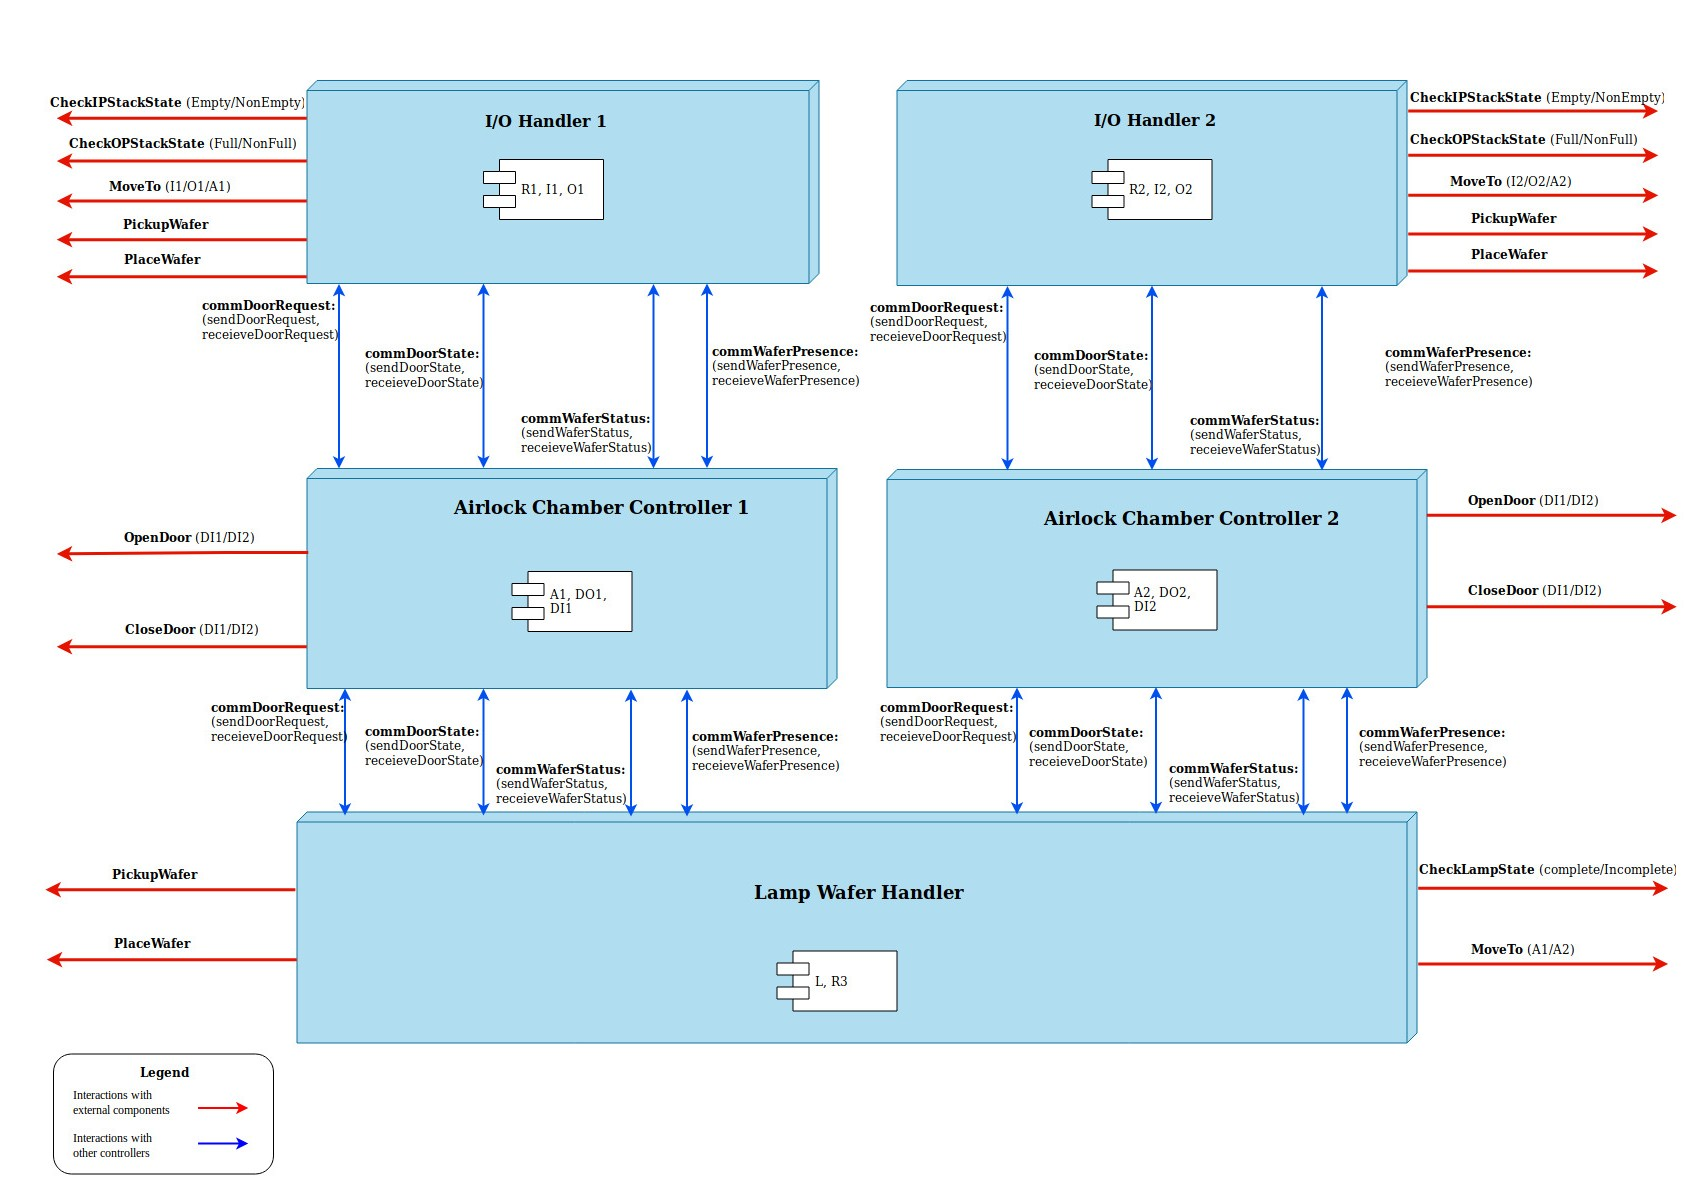
\includegraphics[width=19cm, height=15cm]{Architecture-final.jpg}}
  \caption{Architecture Diagram of System}
  \label{fig:arch1}
\end{figure}
\newpage
\section{Translated Requirements}
\subsection{Introduction}
The requirements mentioned in Section 2 describe what is needed and expected out of the system. A successful verification of the system which conforms to the aforementioned specifications and requirements is to be carried out. This necessitates the use of Modal $\mu$-Calculus.   
\subsection{Modal $\mu$-Calculus}
%\\In order to translate the requirements into their corresponding MCF representations, the requirements are rephrased as follows:
Here the corresponding Modal $\mu$ -Calculus are described:
\begin{enumerate}
%1
\item Once a wafer is picked up from an Input Stack, it eventually gets printed and placed on the Output Stack if the Output Stack is not full. (\textbf{As long as the wafer can move through the production process, it will.}) \textbf{[Liveness]}
\\
\\\textbf{Formula:} $[true*] \forall IP: IPStackID.[CheckIPStackState(IP, Empty).
\\(\overline{MoveTo(MapIPDestination(IP)}*].true$ \\\textbf{Status:}Verified true.

%2
\item Once a wafer is picked up from an Input Stack (I1 or I2), the next wafer from that Input Stack gets picked up only after the previous wafer has been printed and placed on the corresponding Output Stack. \textbf{[Safety]}
\\
\\\textbf{Formula:} $[true*] \forall OP: OPStackID.[CheckOPStackState(OP, Full).
\\(\overline{MoveTo(MapOPDestination(OP)}*].true$ \\\textbf{Status:}Verified true.

%3
\item The Outer Robots (R1 and R2) should not place a wafer on the Input Stacks (I1 and I2). \textbf{[Safety]}
\\
\\\textbf{Formula:} $[true*] \forall IP: IPStackID.[CheckIPStackState(IP, Empty).
\\(\overline{MoveTo(MapIPDestination(IP)}*].true$ \\\textbf{Status:}Verified true.

%4
\item The Outer Robots (R1 and R2) should not pickup a wafer from an empty Input Stack. \textbf{[Safety]}
\\
\\\textbf{Formula:} $[true*] \forall IP: IPStackID.[CheckIPStackState(IP, Empty).
\\(\overline{MoveTo(MapIPDestination(IP)}*].true$ \\\textbf{Status:}Verified true.

%5
\item Once an \textbf{unprocessed} wafer is picked up from its Input Stack by the Outer Robots (R1 and R2), it gets placed in it's corresponding Airlock. \textbf{[Liveness]}
\\
\\\textbf{Formula:} $[true*] \forall IP: IPStackID.[CheckIPStackState(IP, Empty).
\\(\overline{MoveTo(MapIPDestination(IP)}*].true$ \\\textbf{Status:}Verified true.

%6
\item The Outer Robots (R1 and R2) must not pickup an \textbf{unprocessed} wafer from the Airlocks (AL1 and AL2). \textbf{[Safety]}
\\
\\\textbf{Formula:} $[true*] \forall IP: IPStackID.[CheckIPStackState(IP, Empty).
\\(\overline{MoveTo(MapIPDestination(IP)}*].true$ \\\textbf{Status:}Verified true.

%7
\item The Outer and Inner Doors of the Airlocks must not be opened at the same time \textbf{[Safety]}
\begin{enumerate}
    \item The Inner Door (DI1) must not be opened if the Outer Door(DO1) is open for Airlock (AL1).

    \item The Inner Door (DI2) must not be opened if the Outer Door(DO2) is open for Airlock (AL2).

    \item The Outer Door (DO1) must not be opened if the Inner Door(DI1) is open for Airlock (AL1).

    \item The Outer Door (DO2) must not be opened if the Inner Door(DI2) is open for Airlock (AL2).
\end{enumerate}
    \begin{itemize}
	\item \textbf{Formula:} $[true*].[MoveTo(I1).(\overline{MoveTo(AL1}*.MoveTo(O1)].false$ \\\textbf{Status:}Verified true.
    \item \textbf{Formula:} $[true*].[MoveTo(I2).(\overline{MoveTo(AL2}*.MoveTo(O2)].false$ \\\textbf{Status:}Verified true.
	\end{itemize}

%8
\item Once an \textbf{unprocessed} wafer is picked up from an Airlock by the Inner Robot (R3), the wafer gets placed on the Lamp. \textbf{[Liveness]}
\\
\\\textbf{Formula:} $[true*] \forall IP: IPStackID.[CheckIPStackState(IP, Empty).
\\(\overline{MoveTo(MapIPDestination(IP)}*].true$ \\\textbf{Status:}Verified true.
%%%
%9
\item The Inner Robot (R3) will only pickup a \textbf{finished} i.e. printed wafer from the Lamp (L). \textbf{[Safety]}
\\
\\\textbf{Formula:} $[ \overline{CheckLampState(Complete)}^*.PickupWafer(R3,Lamp)]  false$ 
\\\textbf{Status:}Verified true.
%[!CheckLampState(Complete)*.PickupWafer(R3,Lamp)] false
%%%
%10
\item The Inner Robot (R3) will not place the \textbf{finished} wafer again on the Lamp (L). \textbf{[Safety]}
\\
\\\textbf{Formula:} $[true^*.PickupWafer(R3,Lamp).
\\ \overline{PlaceWafer(R3,A1) \vee PlaceWafer(R3,A2)}^*.PlaceWafer(R3,Lamp)] false$ \\\textbf{Status:}Verified true.
%[true*.PickupWafer(R3,Lamp).!(PlaceWafer(R3,A1) || PlaceWafer(R3,A2))*.PlaceWafer(R3,Lamp)] false
%%%
%11
\item Once a \textbf{finished} wafer is picked up from the Lamp by the Inner Robot (R3), the wafer gets placed in its corresponding Airlock. \textbf{[Liveness]}
\\
\\\textbf{Formula:} 
\\\textbf{Status:}Verified true.
%
%%%
%12
\item The Inner Robot (R3) should not pickup a \textbf{processed} wafer from the Airlocks. \textbf{[Safety]}
\\
\\\textbf{Formula:} $[true^*. receiveWaferStatus(AL1, Finished). true^*. 
\\PickupWafer(R3, A1)] false $
\\\textbf{Status:}Verified true.
%[true* . receiveWaferStatus(AL1, Finished). true*. PickupWafer(R3, A1)]false
%%%
%13
\item Once a \textbf{finished} wafer is picked up from an Airlock by the Outer Robots (R1 and R2), the wafer gets placed on it's corresponding Output Stack. \textbf{[Liveness]}
\\
\\\textbf{Formula:} 
\\\textbf{Status:}Verified true.
%
%%%
%14
\item The Outer Robots (R1 and R2) should not pickup a wafer from the Output Stacks (O1 and O2). \textbf{[Safety]}
\begin{enumerate}
\item \textbf{Formula:} $[true^* . PickupWafer(R1, O1)] false$
\\\textbf{Status:}Verified true.
\item \textbf{Formula:} $[true^* . PickupWafer(R2, O2)] false$
\\\textbf{Status:}Verified true.
\end{enumerate}
%[true* . PickupWafer(R1, O1)] false 
%[true* . PickupWafer(R2, O2)] false 
%%%
%15
\item The Outer Robots (R1 and R2) should not place a wafer on the Output Stacks if the Output Stacks are Full. \textbf{[Safety]}
\begin{enumerate}

\item \textbf{Formula:} $[true^* . CheckOPStackState(OP1,Full). \\\overline{CheckOPStackState(OP1, NonFull)}^* .PlaceWafer(R1, O1)] false $
\\\textbf{Status:}Verified true.

\item \textbf{Formula:} $[true^* . CheckOPStackState(OP2,Full). \\\overline{CheckOPStackState(OP2, NonFull)}^* .PlaceWafer(R2, O2)] false $
\\\textbf{Status:}Verified true.
\end{enumerate}
%[true* .CheckOPStackState(OP1,Full). (!CheckOPStackState(OP1, NonFull))* . PlaceWafer(R1, O1)] false 
%[true* .CheckOPStackState(OP2,Full). (!CheckOPStackState(OP2, NonFull))* . PlaceWafer(R2, O2)] false 
%%%
%16
\item The Outer Robots (R1 and R2) should not place an \textbf{unprocessed} wafer on the Output Stacks (O1 and O2). \textbf{[Safety]}
\begin{enumerate}

\item \textbf{Formula:} $[true^* . PickupWafer(R1, I1) .\overline{PickupWafer(R1, A1)}^* . 
\\PlaceWafer(R1, O1)] false $
\\\textbf{Status:}Verified true.

\item \textbf{Formula:} $[true^* . PickupWafer(R2, I2) .\overline{PickupWafer(R2, A2)}^* . 
\\PlaceWafer(R1, O1)] false $
\\\textbf{Status:}Verified true.

\end{enumerate}
%[true* .PickupWafer(R1, I1) .(!PickupWafer(R1, A1))* . PlaceWafer(R1, O1)] false 
%[true* .PickupWafer(R2, I2) .(!PickupWafer(R2, A2))* . PlaceWafer(R2, O2)] false 
%%%
%17
\item \textbf{The system is deadlock free}. \textbf{[Safety]}
\\
\\\textbf{Formula:} $[true^*]. <true> . true$
\\\textbf{Status:}Verified true.
\end{enumerate}
%-------------------------------------%

\newpage
\section{Modelling the System}
\subsection{Component Description}
Our Model consists of the following Components:
\begin{itemize}
    \item 2 IO Handlers which control the (Outer)Robots R1 and R2 and their interactions with the pair of Stacks and the Airlocks.
    \item 2 Airlock Controllers which control the actuation of the Doors and the Airlocks' interactions with the rest of the system.
    \item 1 Lamp Handler which controls the (Inner)Robot R3 and its' interactions with the Lamp and the Airlocks.
\end{itemize}
Currently the two controllers called IO Handler 1 and IO Handler 2 are working in parallel with 2 separate Airlock Controllers for each Airlock and with the Lamp Handler. This results in a system with five parallel components working to move the wafer along the production process. 
\subsection{Initial State}
The system in its initial state has the following configuration:
\begin{itemize}
    \item The Output Stacks start with having no wafers present(empty). The Input Stacks are assumed to have wafers present (non-empty).
    \item The Airlocks don't have any wafer already present in them. All of the Doors of both the Airlocks are closed.
    \item The Lamp does not have any wafer present on it.
\end{itemize} 
The Input The system currently has 87 levels, 1740 states and 3776 transitions.
\subsection{Restrictions and Extensions}
We have however, restricted the controllers to only control and interact with one half of the symmetrical system. This implies that the IO Handlers and Airlock Controllers only interact with a single robot (R1 or R2), single pair of Input and Output stack (I1,O1 or I2,O2), Airlocks (AL1 or AL2) and the corresponding pair of doors (DO1,DI1 or DO2,DI2). This simplifies the system to a great extent and helps in it's modelling.
\\
\\There is a caveat that this simplification will reduce the throughput of the system. This happens when one of the Stacks no longer have wafers present but the other pair of stacks still do. Hence, as an extension, we have considered the possibility of modelling a system which will have the flexibility to move the robots to different stacks and hence increase the throughput. 
We have considered the case when the output stacks are emptied once they are full and the case when the input stacks are replenished. Our system loops around the check for the stacks to return to a workable state (Input not empty and Output not full)
\begin{figure}[ht]
\centering
    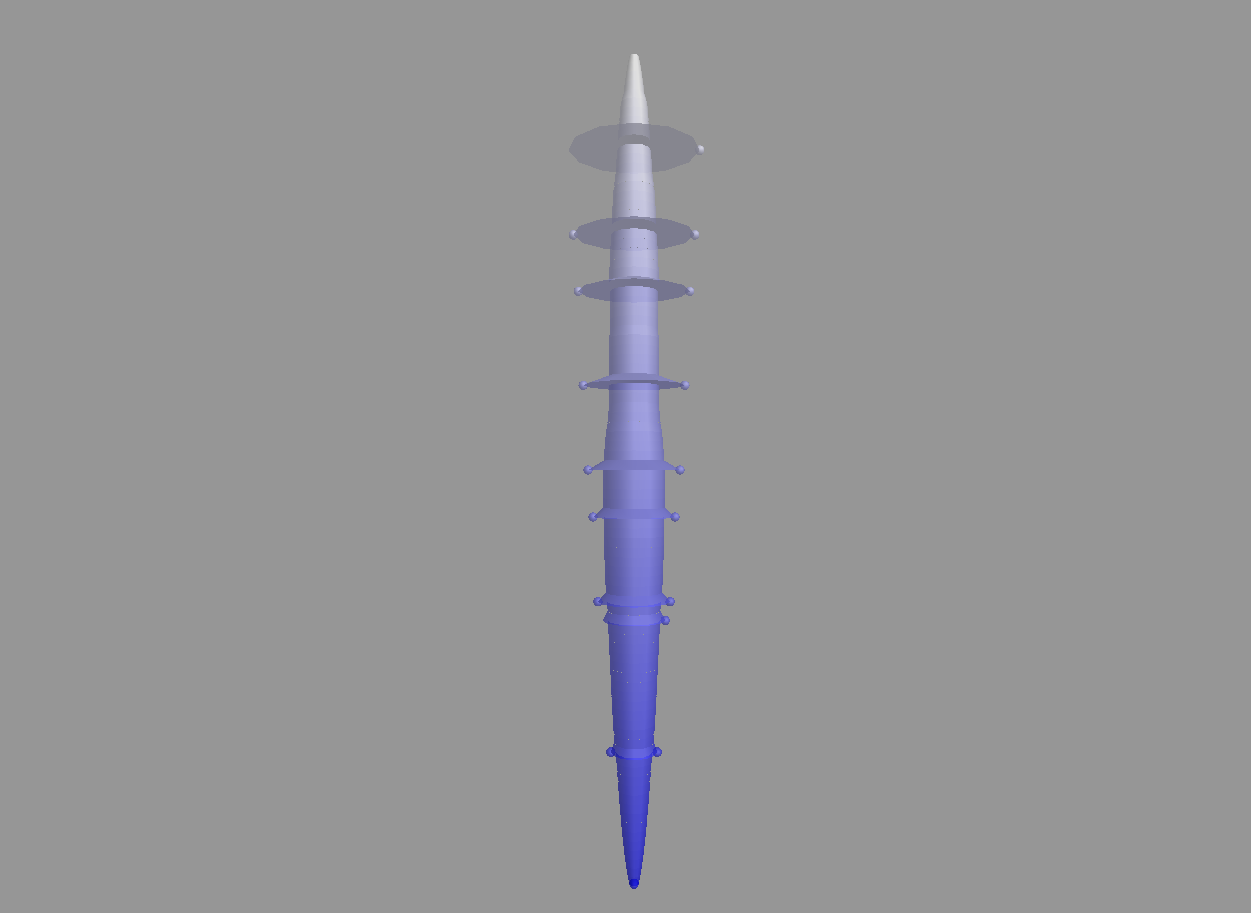
\includegraphics[width=\textwidth, height=8cm]{3D-Model.png}
  \caption{LTSView of the System}
  \label{fig:ltsview}
\end{figure}
\newpage
\section{Verification}
The Verification process involved three main steps. We created a simplified version of the model where only a single IO Handler, Airlock Controller and Lamp Handler was present. We disregarded the second pair of Input Output Stacks along with the Robot and Airlock. This way we could visualize the system using LTSGraph. This worked well because we needed to identify the cause for the deadlock occurring in our system. We used LPSxSim simulation to logically verify the correct sequence of actions for the process (only for the simplified system). Once we corrected the mistake and cleared the deadlocking condition, we used the complete, more complex system for all of our verification.
\\
\\The Complete Model was visually inspected using LTSView to mark for deadlocks.These are presented in the Visualization subsection. The $\mu$ Calculus derived from the translated requirements from Section 5 are presented in Appendix B 
\subsection{Tools}
In order to replicate our results, we provide the exact version of the tools we used along with the system configuration we used them on.
\\
\\The following version of mcrl2 was used:
\begin{itemize}
    \item mcrl2 --version: 201808.0
\end{itemize}
The following tools were used for modelling and verification: mcrl2xi, mcrl22lps, lpsxsim, lps2lts, ltsgraph, ltsview, lts2pbes, pbessolve.
\\The following is the specification of the system used for the above tools:
\begin{itemize}
    \item Windows 10, Intel i-core i7, 2.8GHz processor with 16GB RAM 
\end{itemize}
\subsection{Verification Checks}
The method used for formal verification of the system requirements presented in Section 2 is converting the model to PBES and then verifying each Modal $\mu$ Formula individually. The formulae for Modal $\mu$ Calculus presented in Section 5 have been verified individually and each of the formula holds true for the model presented.
\subsection{Visualizations}
The visual representations provide an additional guide to verify that the system is, indeed, deadlock free. Figure \ref{fig:ltsview-1} shows the system when visualized with LTSView tool. The figure represents the states and transitions present in the model. Figure \ref{fig:deadlockfree} shows the model when marked for deadlocks. The absence of red dots confirms that the system is deadlock free.
\begin{figure}[ht]
    \centering
    \begin{minipage}{0.45\textwidth}
        \centering
        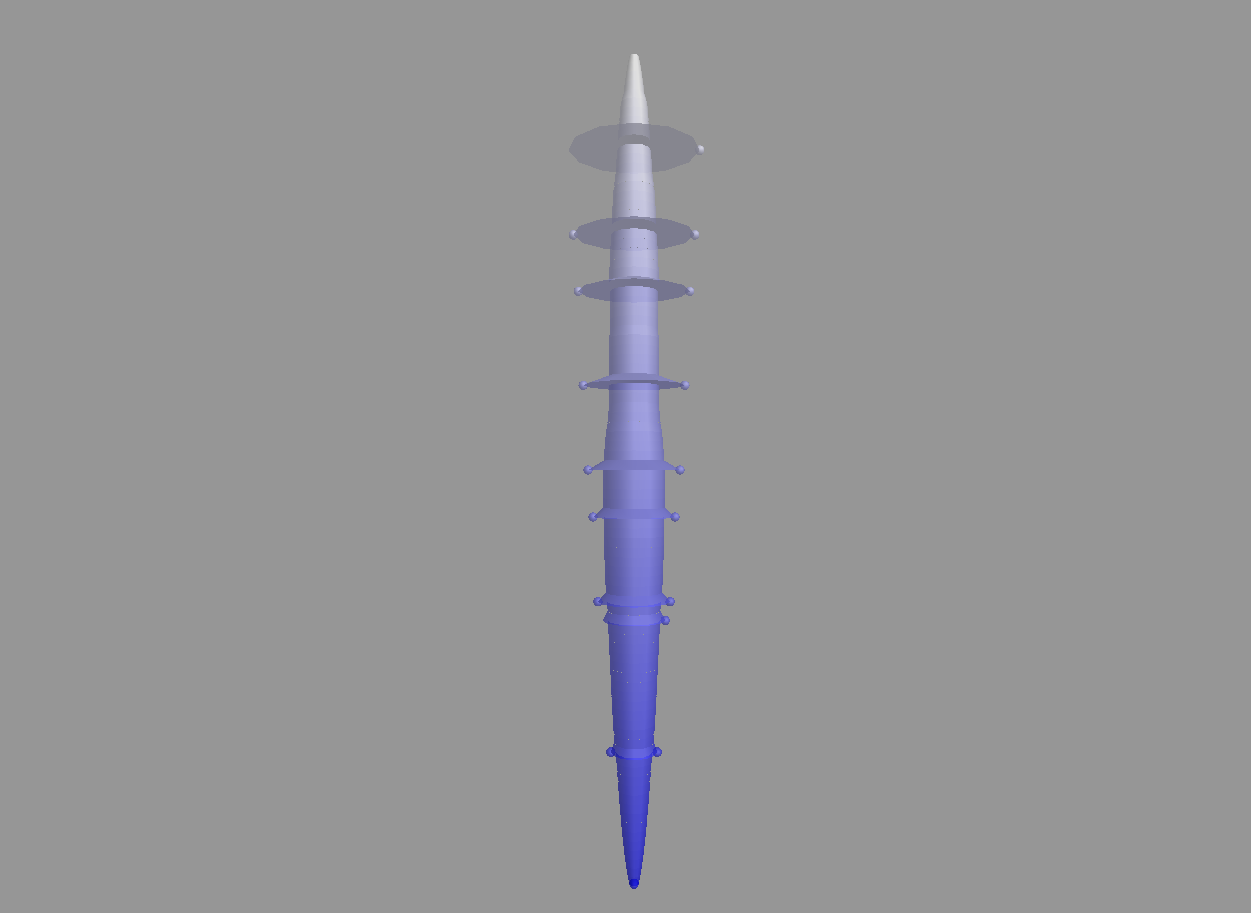
\includegraphics[width=0.9\textwidth]{3D-Model.png} \caption{LTSView}
        \label{fig:ltsview-1}
    \end{minipage}\hfill
    \begin{minipage}{0.45\textwidth}
        \centering
        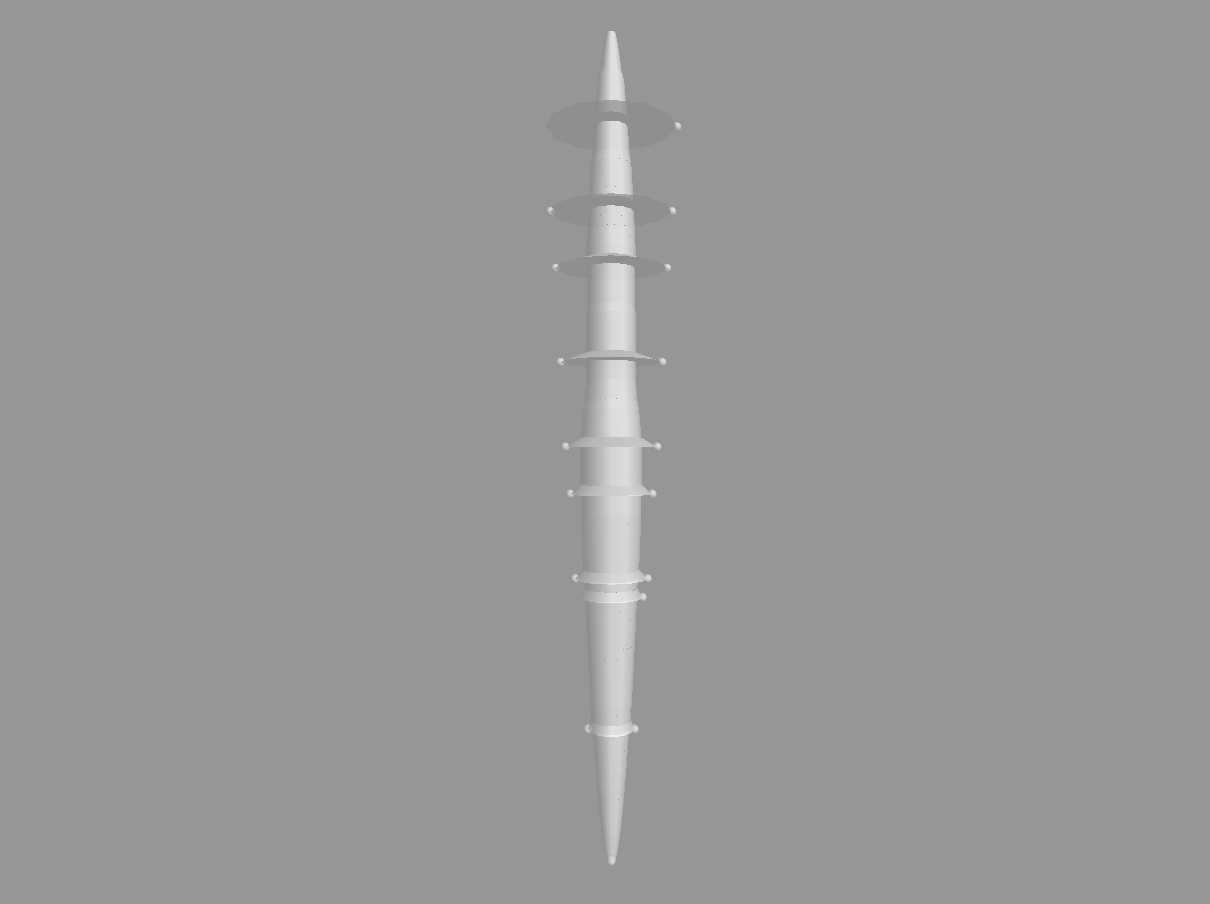
\includegraphics[width=0.9\textwidth]{Deadlockfree.png} 
        \caption{Marking Deadlocks}
        \label{fig:deadlockfree}
    \end{minipage}
\end{figure}
\newpage
\section{Conclusion}
As part of the given assignment, we have modelled a Wafer production system as described in the assignment prompt. This project consisted of multiple phases. In the first phase the system components were determined and requirements were formalized. In the second phase the interactions between the systems and the communications between different controllers were defined. Based on the system components along with the formulated requirements and interactions an architecture was developed. The third phase involved modelling with the mcrl2 tool. In the fourth phase requirements were translated into $\mu$-calculus Calculus. In the fifth phase the model was verified by translating the $\mu$-calculus Calculus from phase 4 into Modal $\mu$-Code. 

\newpage
\appendix
\section{Code: mcrl2}
\textbf{sort} LocationID = \textbf{struct} A1 $|$ A2 $|$ I1 $|$ I2 $|$ O1 $|$ O2 $|$ Lamp;
\\		  StackID = \textbf{struct} IP1 $|$ IP2 $|$ OP1 $|$ OP2;
\\		  AirlockID = \textbf{struct} AL1 $|$ AL2 $|$ None;
\\     IOHandlerID = \textbf{struct} IOH1 $|$ IOH2;
\\		  OperationType = \textbf{struct} Get $|$ Put;
\\		  IPStackState = \textbf{struct} Empty $|$ NonEmpty;
\\		  OPStackState = \textbf{struct} Full $|$ NonFull;
\\	    DoorID = \textbf{struct} DI1 $|$ DI2 $|$ DO1 $|$ DO2;		
\\		  DoorState = \textbf{struct} Open $|$ Closed;
\\			LampState = \textbf{struct} Incomplete $|$ Complete;
\\		  CycleType = \textbf{struct} Input $|$ Output;
\\		  WaferType = \textbf{struct} New $|$ Finished $|$ NoWafer;
\\
\\\textbf{map} CorrespondingDoor : DoorID -> DoorID;
\\	  CorrespondingOPDestination : IPStackID -> \\DestinationID;		
\\	  MapOPDestination : OPStackID -> DestinationID;
\\		MapIPDestination : IPStackID -> DestinationID;
\\		MapAirlock : AirlockID -> DestinationID;
\\
\\ \textbf{eqn} CorrespondingDoor(DO1) = DI1;
\\		CorrespondingDoor(DI1) = DO1;
\\		CorrespondingDoor(DO2) = DI2;
\\		CorrespondingDoor(DI2) = DO2;
\\
\\		CorrespondingOPDestination(IP1) = O1;
\\		CorrespondingOPDestination(IP2) = O2;
\\
\\		MapOPDestination(OP1) = O1;
\\		MapOPDestination(OP2) = O2;
\\		MapIPDestination(IP1) = I1;
\\		MapIPDestination(IP2) = I2;
\\
\\		MapAirlock(AL1) = A1;
\\		MapAirlock(AL2) = A2;
\\		MapAirlock(None) = Null;
\\
\\\textbf{act} MoveTo: DestinationID;
\\	  PickupWafer;
\\	  PlaceWafer;
\\
\\	    OpenDoor : DoorID;
\\		CloseDoor : DoorID;
\\
\\	  CheckIPStackState : StackID \# IPStackState;
\\	  CheckOPStackState : StackID \# OPStackState;
\\		CheckLampState : LampState;
\\
\\	  receiveDoorState : DoorID \# DoorState;
\\	  sendDoorState : DoorID \# DoorState;
\\		commDoorState : DoorID \# DoorState;
\\
\\	  receiveDoorRequest : DoorID \# DoorState;
\\		sendDoorRequest : DoorID \# DoorState;
\\		commDoorRequest : DoorID \# DoorState;
\\
\\	  receiveWaferStatus : AirlockID \# WaferType;
\\		sendWaferStatus : AirlockID \# WaferType;
\\		commWaferStatus : AirlockID \# WaferType;
\\
\\	  receiveWaferPresence : AirlockID \# WaferType;
\\		sendWaferPresence : AirlockID \# WaferType;
\\		commWaferPresence : AirlockID \# WaferType;
\\
\\
\\\textbf{proc} IOHandler1(Operation : OperationType, Cycle : CycleType) = 
\\((Cycle == Input) \&\& (Operation == Get)) -$>$ CheckIPStackState(IP1,Empty)
\\.IOHandler1(Operation = Get)
\\
\\+ ((Cycle == Input) \&\& (Operation == Get)) -$>$ CheckIPStackState(IP1,NonEmpty)
\\.MoveTo(I1).PickupWafer.IOHandler1(Operation = Put)
\\
\\+ ((Cycle == Input) \&\& (Operation == Put)) -$>$ receiveDoorState(DO1,Closed)
\\.sendDoorRequest(DO1,Open).IOHandler1(Operation = Put)
\\
\\+ ((Cycle == Input) \&\& (Operation == Put)) -$>$ receiveDoorState(DO1,Open)
\\.MoveTo(A1).PlaceWafer.sendWaferStatus(AL1,New).IOHandler1(Cycle = Output, Operation = Get)
\\
\\
\\+ ((Cycle == Output) \&\& (Operation == Get)) -$>$ receiveWaferPresence(AL1,NoWafer).IOHandler1(Operation = Get)
\\
\\+ ((Cycle == Output) \&\& (Operation == Get)) -$>$ receiveWaferPresence(AL1,Finished).receiveDoorState(DO1,Closed).sendDoorRequest(DO1,Open)
.receiveDoorState(DO1,Open).MoveTo(A1).PickupWafer.IOHandler1(Operation = Put)
\\
\\+ ((Cycle == Output) \&\& (Operation == Put)) -$>$ CheckOPStackState(OP1,Full)
\\.IOHandler1(Operation = Put)
\\+ ((Cycle == Output) \&\& (Operation == Put)) -$>$ CheckOPStackState(OP1,NonFull)
\\.MoveTo(O1).PlaceWafer.IOHandler1(Cycle = Input, Operation = Get);
\\
\\IOHandler2(Operation : OperationType, Cycle : CycleType) =
\\((Cycle == Input) \&\& (Operation == Get)) -$>$ CheckIPStackState(IP2,Empty)
\\.IOHandler2(Operation = Get)
\\+ ((Cycle == Input) \&\& (Operation == Get)) -$>$ CheckIPStackState(IP2,NonEmpty)
\\.MoveTo(I2).PickupWafer.IOHandler2(Operation = Put)
\\+ ((Cycle == Input) \&\& (Operation == Put)) -$>$ receiveDoorState(DO2,Closed)
\\.sendDoorRequest(DO2,Open).IOHandler2(Operation = Put)
\\+ ((Cycle == Input) \&\& (Operation == Put)) -$>$ receiveDoorState(DO2,Open)
\\.MoveTo(A2).PlaceWafer.sendWaferStatus(AL2,New).IOHandler2(Cycle = Output, Operation = Get)
\\
\\+ ((Cycle == Output) \&\& (Operation == Get)) -$>$ receiveWaferPresence(AL2,NoWafer).IOHandler2(Operation = Get)
\\+ ((Cycle == Output) \&\& (Operation == Get)) -$>$ receiveWaferPresence(AL2,Finished).receiveDoorState(DO2,Closed).sendDoorRequest(DO2,Open)
.receiveDoorState(DO2,Open)
\\.MoveTo(A2).PickupWafer.IOHandler2(Operation = Put)
\\
\\+ ((Cycle == Output) \&\& (Operation == Put)) -$>$ CheckOPStackState(OP2,Full)
\\.IOHandler2(Operation = Put)
\\+ ((Cycle == Output) \&\& (Operation == Put)) -$>$ CheckOPStackState(OP2,NonFull)
\\.MoveTo(O2).PlaceWafer.IOHandler2(Cycle = Input, Operation = Get);
\\
\\AirlockChamber1Controller(WaferPresence : WaferType, OuterDoorState : DoorState, InnerDoorState : DoorState) =
((OuterDoorState == Closed) \&\& (InnerDoorState == Open)) -$>$ receiveDoorRequest(DO1,Open)
\\.AirlockChamber1Controller(InnerDoorState = Open)
\\
\\+ ((OuterDoorState == Closed) \&\& (InnerDoorState == Closed)) -$>$ receiveDoorRequest(DO1,Open)
\\.OpenDoor(DO1).AirlockChamber1Controller(OuterDoorState = Open)
\\+ ((OuterDoorState == Open) \&\& (InnerDoorState == Closed)) -$>$ receiveDoorRequest(DI1,Open)
\\.AirlockChamber1Controller(OuterDoorState = Open)
\\+ ((OuterDoorState == Closed) \&\& (InnerDoorState == Closed)) -$>$ receiveDoorRequest(DI1,Open)
\\.OpenDoor(DI1).AirlockChamber1Controller(InnerDoorState = Open)
\\
\\+ ((OuterDoorState == Open) \&\& (InnerDoorState == Closed)) -$>$ receiveWaferStatus(AL1,New).CloseDoor(DO1)
\\.AirlockChamber1Controller(WaferPresence = New, OuterDoorState = Closed)
\\+ ((OuterDoorState == Closed) \&\& (InnerDoorState == Open)) -$>$ receiveWaferStatus(AL1,Finished).CloseDoor(DI1)\\.AirlockChamber1Controller(WaferPresence = Finished, InnerDoorState = Closed)
\\
\\+ sendDoorState(DO1,OuterDoorState).AirlockChamber1Controller()
\\+ sendDoorState(DI1,InnerDoorState).AirlockChamber1Controller()
\\+ sendWaferPresence(AL1,WaferPresence).AirlockChamber1Controller();
\\
\\AirlockChamber2Controller(WaferPresence : WaferType, OuterDoorState : DoorState, InnerDoorState : DoorState) =
((OuterDoorState == Closed) \&\& (InnerDoorState == Open)) -$>$ receiveDoorRequest(DO2,Open)
\\.AirlockChamber2Controller(InnerDoorState = Open)
\\+ ((OuterDoorState == Closed) \&\& (InnerDoorState == Closed)) -$>$ receiveDoorRequest(DO2,Open)
\\.OpenDoor(DO2).AirlockChamber2Controller(OuterDoorState = Open)
\\+ ((OuterDoorState == Open) \&\& (InnerDoorState == Closed)) -$>$ receiveDoorRequest(DI2,Open)
\\.AirlockChamber2Controller(OuterDoorState = Open)
\\+ ((OuterDoorState == Closed) \&\& (InnerDoorState == Closed)) -$>$ receiveDoorRequest(DI2,Open)
\\.OpenDoor(DI2).AirlockChamber2Controller(InnerDoorState = Open)
\\
\\+ ((OuterDoorState == Open) \&\& (InnerDoorState == Closed)) -$>$ receiveWaferStatus(AL2,New).CloseDoor(DO2)
\\.AirlockChamber2Controller(WaferPresence = New, OuterDoorState = Closed)
\\+ ((OuterDoorState == Closed) \&\& (InnerDoorState == Open)) -$>$ receiveWaferStatus(AL2,Finished).CloseDoor(DI2)\\.AirlockChamber2Controller(WaferPresence = Finished, InnerDoorState = Closed)
\\
\\+ sendDoorState(DO2,OuterDoorState).AirlockChamber2Controller()
\\+ sendDoorState(DI2,InnerDoorState).AirlockChamber2Controller()
\\+ sendWaferPresence(AL2,WaferPresence).AirlockChamber2Controller();
\\
\\LampWaferHandler(Cycle : CycleType, CurrentAirlock : AirlockID) = 
\\
\\((Cycle == Input) \&\& (CurrentAirlock == None)) -$>$ receiveWaferPresence(AL1,New).LampWaferHandler(CurrentAirlock = AL1)
\\+ ((Cycle == Input) \&\& (CurrentAirlock == AL1)) -$>$ receiveDoorState(DI1,Closed)
\\.sendDoorRequest(DI1,Open).LampWaferHandler(CurrentAirlock = AL1)
\\+ ((Cycle == Input) \&\& (CurrentAirlock == AL1)) -$>$ receiveDoorState(DI1,Open)
\\.MoveTo(A1).PickupWafer.MoveTo(Lamp).PlaceWafer.LampWaferHandler(Cycle = Output)
\\
\\+ ((Cycle == Output) \&\& (CurrentAirlock == AL1)) -$>$ CheckLampState(Incomplete).LampWaferHandler(Cycle = Output)
\\
\\+ ((Cycle == Output) \&\& (CurrentAirlock == AL1)) -$>$ CheckLampState(Complete).MoveTo(Lamp).PickupWafer
\\.MoveTo(A1).PlaceWafer.sendWaferStatus(AL1,Finished).LampWaferHandler(Cycle = Input, CurrentAirlock = None)
\\
\\+ ((Cycle == Input) \&\& (CurrentAirlock == None)) -$>$ receiveWaferPresence(AL2,New).LampWaferHandler(CurrentAirlock = AL2)
\\
\\+ ((Cycle == Input) \&\& (CurrentAirlock == AL2)) -$>$ receiveDoorState(DI2,Closed)
\\.sendDoorRequest(DI2,Open).LampWaferHandler(CurrentAirlock = AL2)
\\
\\+ ((Cycle == Input) \&\& (CurrentAirlock == AL2)) -$>$ receiveDoorState(DI2,Open)\\.MoveTo(A2).PickupWafer.MoveTo(Lamp).PlaceWafer.LampWaferHandler(Cycle = Output)
\\
\\+ ((Cycle == Output) \&\& (CurrentAirlock == AL2)) -$>$ CheckLampState(Incomplete).LampWaferHandler(Cycle = Output)
\\
\\
\\
\\
\\+ ((Cycle == Output) \&\& (CurrentAirlock == AL2)) -$>$ CheckLampState(Complete).MoveTo(Lamp).PickupWafer.MoveTo(A2).PlaceWafer
\\.sendWaferStatus(AL2,Finished).LampWaferHandler(Cycle = Input, CurrentAirlock = None);
\\
\\\textbf{init} 
\\
\\\textbf{			allow}(
\\						{MoveTo,
 \\ 				 	 PickupWafer,
 \\				 		 PlaceWafer,
 \\	    			 CheckIPStackState,
\\	  				 CheckOPStackState,
\\						 CheckLampState,
\\						 OpenDoor,
\\						 CloseDoor,
\\
\\						 commDoorState,
\\						 commDoorRequest,
\\						 commWaferStatus,
\\						 commWaferPresence},
\\
\\\textbf{			comm}(
\\						{receiveDoorState $|$ sendDoorState -$>$ commDoorState,
\\						receiveDoorRequest $|$ sendDoorRequest -$>$ commDoorRequest,
\\	  				 	receiveWaferStatus $|$ sendWaferStatus -$>$ commWaferStatus,
\\				 	   receiveWaferPresence $|$ sendWaferPresence -$>$ commWaferPresence},
\\
\\						 IOHandler1(Get, Input) $|$ $|$ IOHandler2(Get, Input) $|$ $|$ AirlockChamber1Controller(NoWafer, Closed, Closed) $|$ $|$ AirlockChamber2Controller(NoWafer, Closed, Closed) $|$ $|$ LampWaferHandler(Input,None)
\\					 ));
\newpage
\section{Code: $\mu$-Calculus}
\begin{enumerate}

\item mcrl2 MCF: [true*] forall IP : IPStackID . [ CheckIPStackState(IP,Empty).
\\(!MoveTo(MapIPDestination(IP)))* ] true

\item mcrl2 MCF: [true*] forall OP : OPStackID . [ CheckOPStackState(OP,Full).
\\(!MoveTo(MapOPDestination(OP)))* ] true

%\item mcrl2 MCF:

\item mcrl2 MCF: (a) [true*] [MoveTo(MapIPDestination(IP1)). (!MoveTo(MapAirlock(AL1)))*
\\.MoveTo(MapOPDestination(OP1))] false
\\
\\ (b) [true*] [MoveTo(MapIPDestination(IP2)). (!MoveTo(MapAirlock(AL2)))*.MoveTo(MapOPDestination(OP2))] false

%\item mcrl2 MCF: [true*] forall IP : IPStackID.[MoveTo(MapIPDestination(IP))] [PlaceWafer] false

%\item mcrl2 MCF:

%\item mcrl2 MCF:

\item mcrl2 MCF: [true*] forall d : DoorID . [ OpenDoor(d).(!CloseDoor(d))*
\\.OpenDoor(CorrespondingDoor(d)) ] false

\item mcrl2 MCF: [true*] forall d : DoorID . [ OpenDoor(d).(!CloseDoor(d))*
\\.OpenDoor(CorrespondingDoor(d)) ] false

\item mcrl2 MCF: [true*] forall d : DoorID . [ OpenDoor(d).(!CloseDoor(d))*
\\.OpenDoor(CorrespondingDoor(d)) ] false

\item mcrl2 MCF: [true*] forall d : DoorID . [ OpenDoor(d).(!CloseDoor(d))*
\\.OpenDoor(CorrespondingDoor(d)) ] false

\item mcrl2 MCF: [true*] forall d : DoorID . [ OpenDoor(d).(!CloseDoor(d))*
\\.OpenDoor(CorrespondingDoor(d)) ] false

\item mcrl2 MCF: [true*.receiveWaferStatus(AL1, Finished). !OpenDoor(DI1)*] true


\item mcrl2 MCF: [true*.receiveWaferStatus(AL1, New). !OpenDoor(DO1)*] true

\item mcrl2 MCF: [true*].<true>.true

\end{enumerate}
\end{document}
